\section{Pruebas}

% Describir como se van a llevar a cabo las pruebas. Hay servicios que se pueden desactivar en las estaciones reales sin afectar gravemente el funcionamiento.
% Se levantó una estación de prueba virtual con X características, la cual es posible apagar la conectividad.

% Qué se hizo, cómo se hizo y como es que funcionaron las pruebas. El driver manda un mensaje de error cuando funcionaron las pruebas, no se puede apagar en estaciones de producción porque perdemos datos.

Una cualidad fundamental del desarrollo ágil son las pruebas contínuas del software que es desarrollado, esto fue llevado a cabo, en parte, gracias a la generación automática del esquema OpenAPI con el que se realizaron pruebas contínuamente del API con la herramienta Insomnia, tal como se muestra en la Figura \ref{fig:insomnia-stations-request}. Con esta herramienta, se corroboró la validez de la información, su estructura y el correcto funcionamiento aún cuando no era posible realizar pruebas del sistema por medio de la interfaz gráfica.

\begin{figure}[!ht]
	\centering
	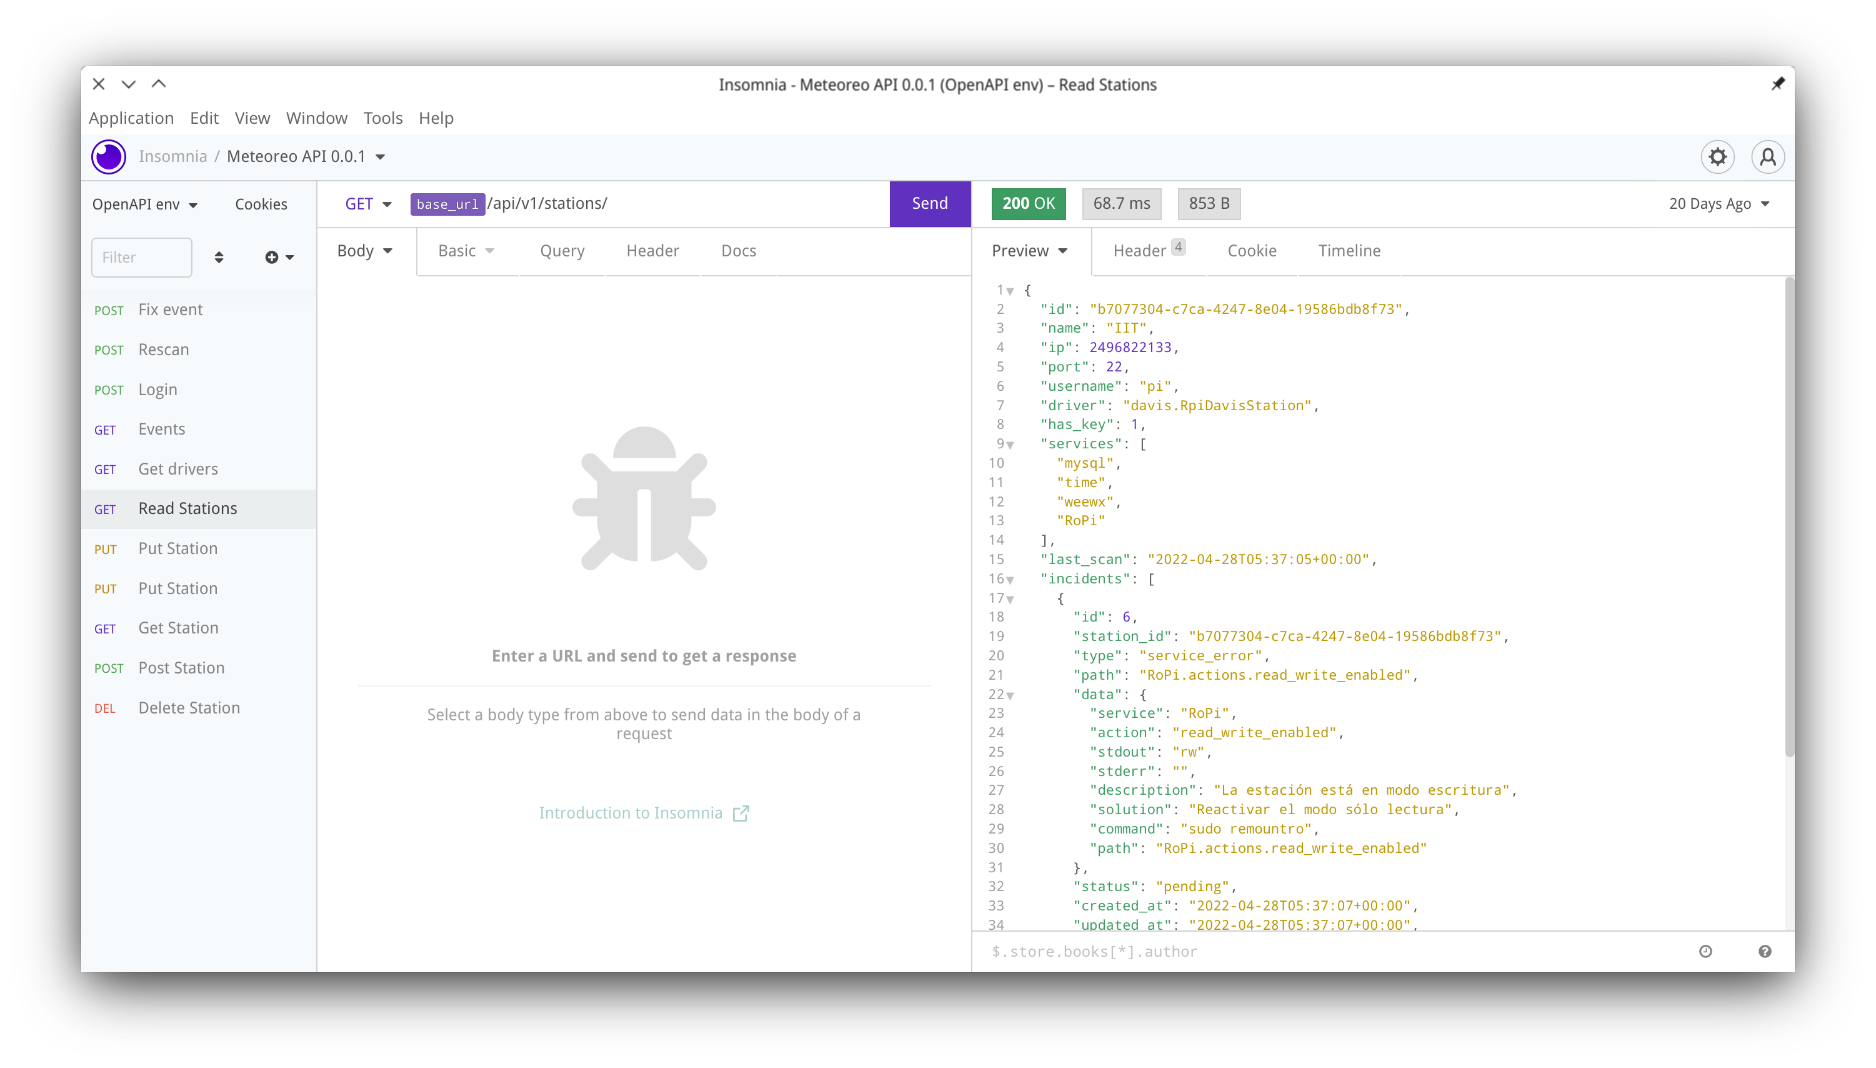
\includegraphics[width=1\linewidth]{images/screenshots/insomnia_stations.png}
	\caption{Solicitud al servidor de pruebas con Insomnia.}
	\label{fig:insomnia-stations-request}
\end{figure}

En preparación para un lanzamiento formal del proyecto, se decidió el realizar múltiples pruebas. Una de estas fue realizada con una estación de prueba para no afectar la recolección de datos de las estaciones instaladas. Para ello se utilizó una imagen de Docker existente con el sistema de WeeWX preconfigurado. Esta imagen posee la peculiaridad de tener instalado el servicio como un módulo de \texttt{systemd}, esto es poco común debido a que las guías de Docker fomentan la replicabilidad y la modularidad de los contenedores \cite{docker_multi_service}, lo cual es incompatible con la configuración seleccionada.

Esta imagen fue utilizada como punto de partida para simular una estación meteorológica, la cual se inició en el ambiente de desarrollo configurado previamente. Para logralo, se creó un comando que ejecutara la imagen de Docker como un proceso en segundo plano, y se adjuntara a la red virtual \texttt{meteoreo-api\_meteoreo-backend}, la cual fue creada automáticamente al iniciar el sistema localmente. La instrucción resultante, que puede ser encontrada en el Listado \ref{lst:test_station_docker}, contiene además de estas especificaciones, configuraciones para el correcto funcionamiento de la imagen y la activación de los servicios SSH.

\begin{listing}
\begin{minted}[%
   breaklines
]{bash}
docker run -td \
   --stop-signal=SIGRTMIN+3 \
   -v /sys/fs/cgroup:/sys/fs/cgroup:rw --cgroupns=host \
   -v /weatherdir:/var/lib/weewx:rw \
   --hostname=weewx \
   --tmpfs /run:size=100M --tmpfs /run/lock:size=100M \
   -e DEBBASE_SSH=enabled \
   --network=meteoreo-api_meteoreo-backend \
   --name=weewx jgoerzen/weewx:4.6.0
\end{minted}
\caption{Funcionamiento de estación de prueba de docker}
\label{lst:test_station_docker}
\end{listing}

Después de haber ejecutado el comando anterior, la imagen ya era accesible desde el ambiente de desarrollo creado con VSCode, y después de resolver inconvenientes que surgieron con la estación al no tener configuraciones adecuadas de SSH fue posible acceder de forma convencional por este protocolo a la estación. Después de verificar la conectividad y su correcto funcionamiento, se registró la por medio de la interfaz gráfica, como se muestra en la Figura \ref{fig:test-station-register}.

\begin{figure}[!ht]
	\centering
	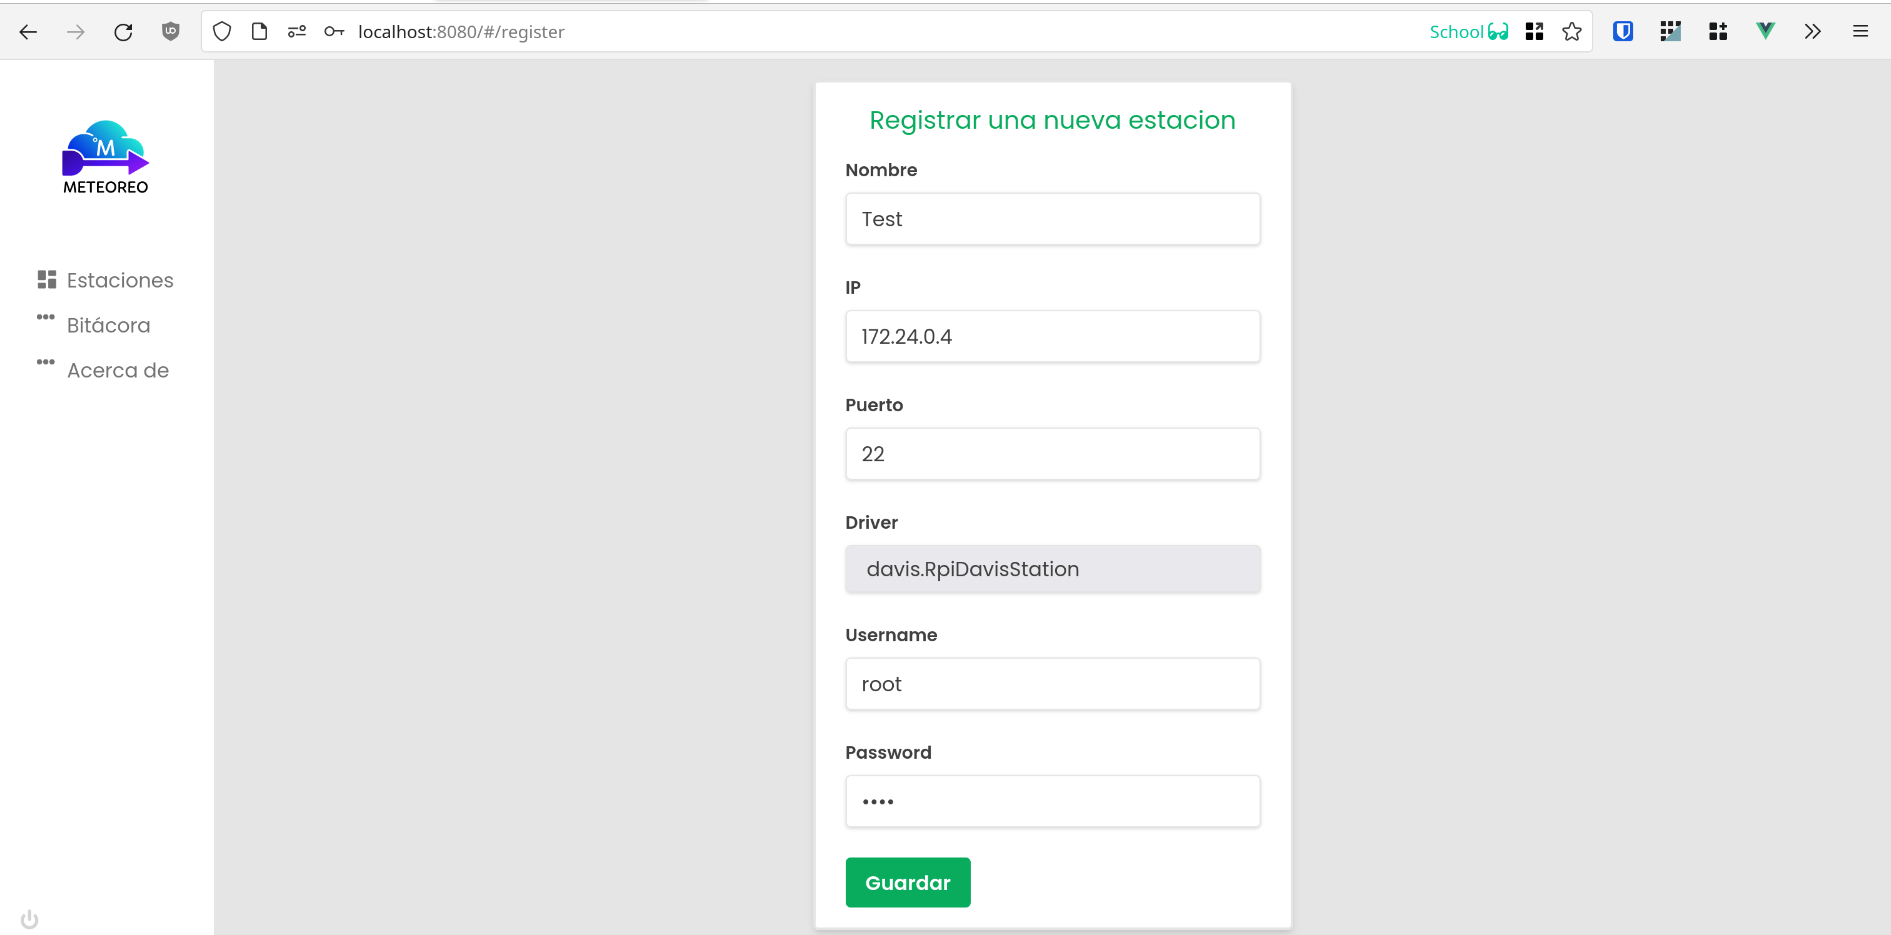
\includegraphics[width=1\linewidth]{images/screenshots/0.1.1-test_station_register.png}
	\caption{Registro de la estación de prueba.}
	\label{fig:test-station-register}
\end{figure}

Al completar el registro de la estación meteorológica, se decidió verificar el correcto funcionamiento del servicio de monitoreo. Al terminar este proceso, era posible observar que la estación tenía 2 fallas, como se muestra en la Figura \ref{fig:test-station-initial}. Estas fallas eran el error del servicio RoPI, la cual era esperada debido a que las limitaciones de Docker impiden volver el sistema raíz como solo escritura; y una falla porque el servicio de MySQL no fue encontrado en la imagen.

\begin{figure}[!ht]
	\centering
	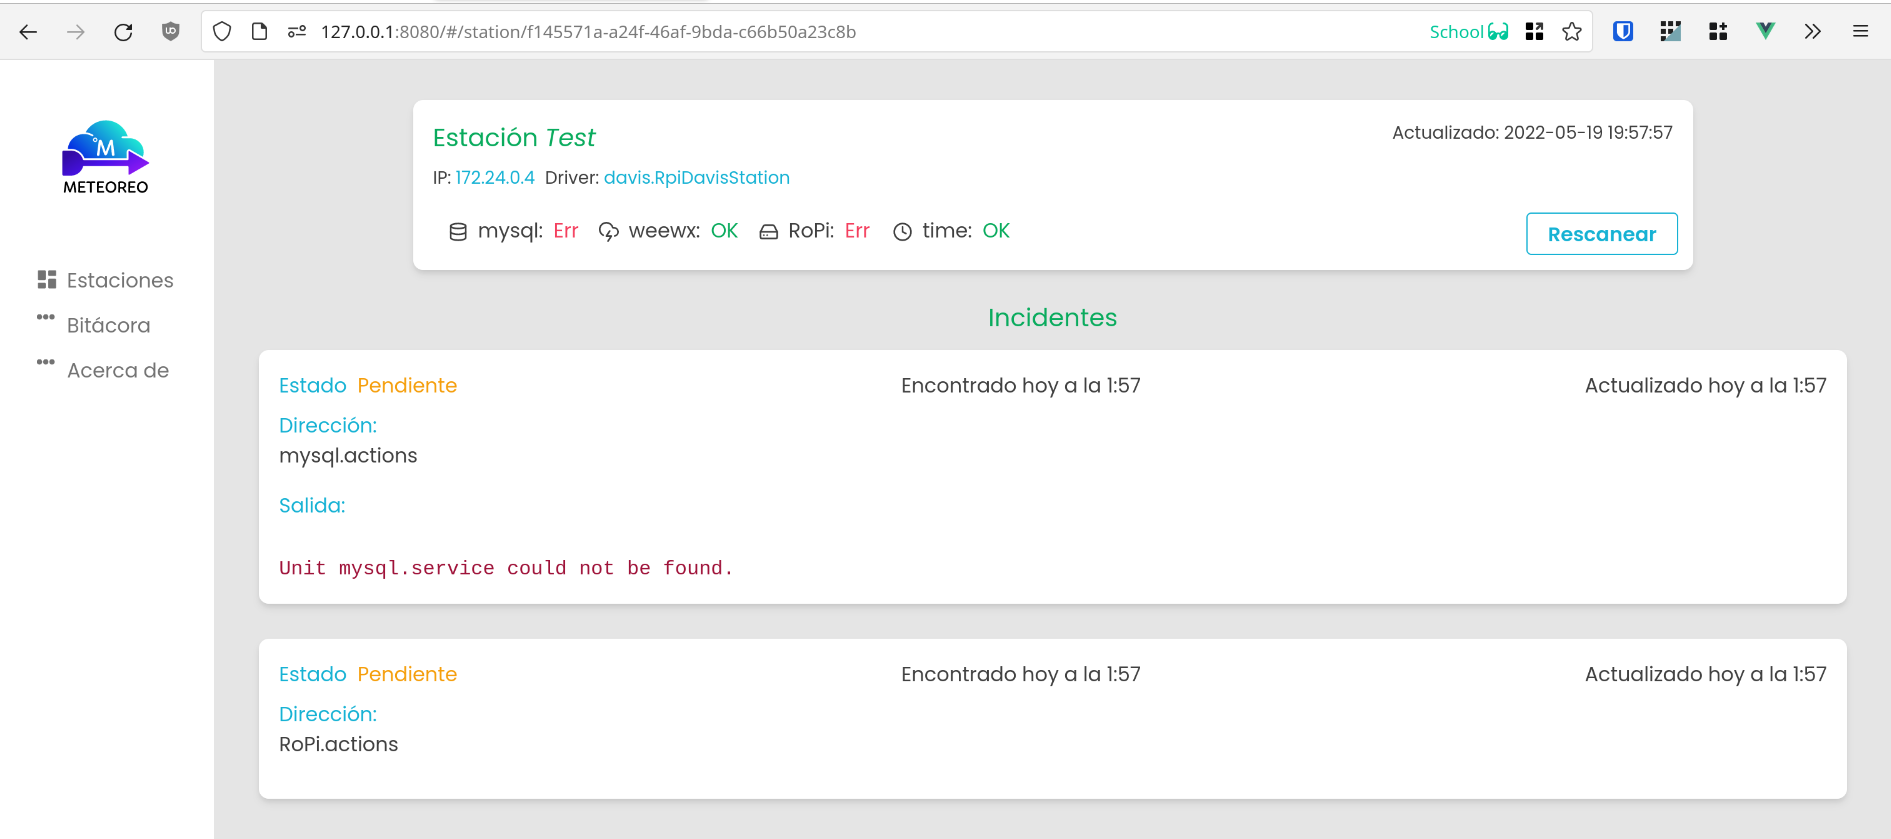
\includegraphics[width=1\linewidth]{images/screenshots/0.1.2-test_station_initial_status.png}
	\caption{Estado incial de la estación de prueba.}
	\label{fig:test-station-initial}
\end{figure}

Esta falla fue solucionada al instalar MySQL en la estación de prueba, lo cual se realizó descargando el paquete correspondiente a la estación del sitio oficial y configurándolo con la utilería de sistema \texttt{dpkg}. Al haber completado este proceso, se volvió a revisar el estado de la estación de acuerdo al servicio de monitoreo, y el resultado esperado fue encontrado.

Después de este proceso de configuración se procedió a realizar la prueba del correcto funcionamiento del servicio de monitoreo. Para ello, se detuvieron los servicios de MySQL y WeeWX en la estación de prueba, el resultado de esta acción puede observarse en la Figura \ref{fig:test-station-failed}.

\begin{figure}[!ht]
	\centering
	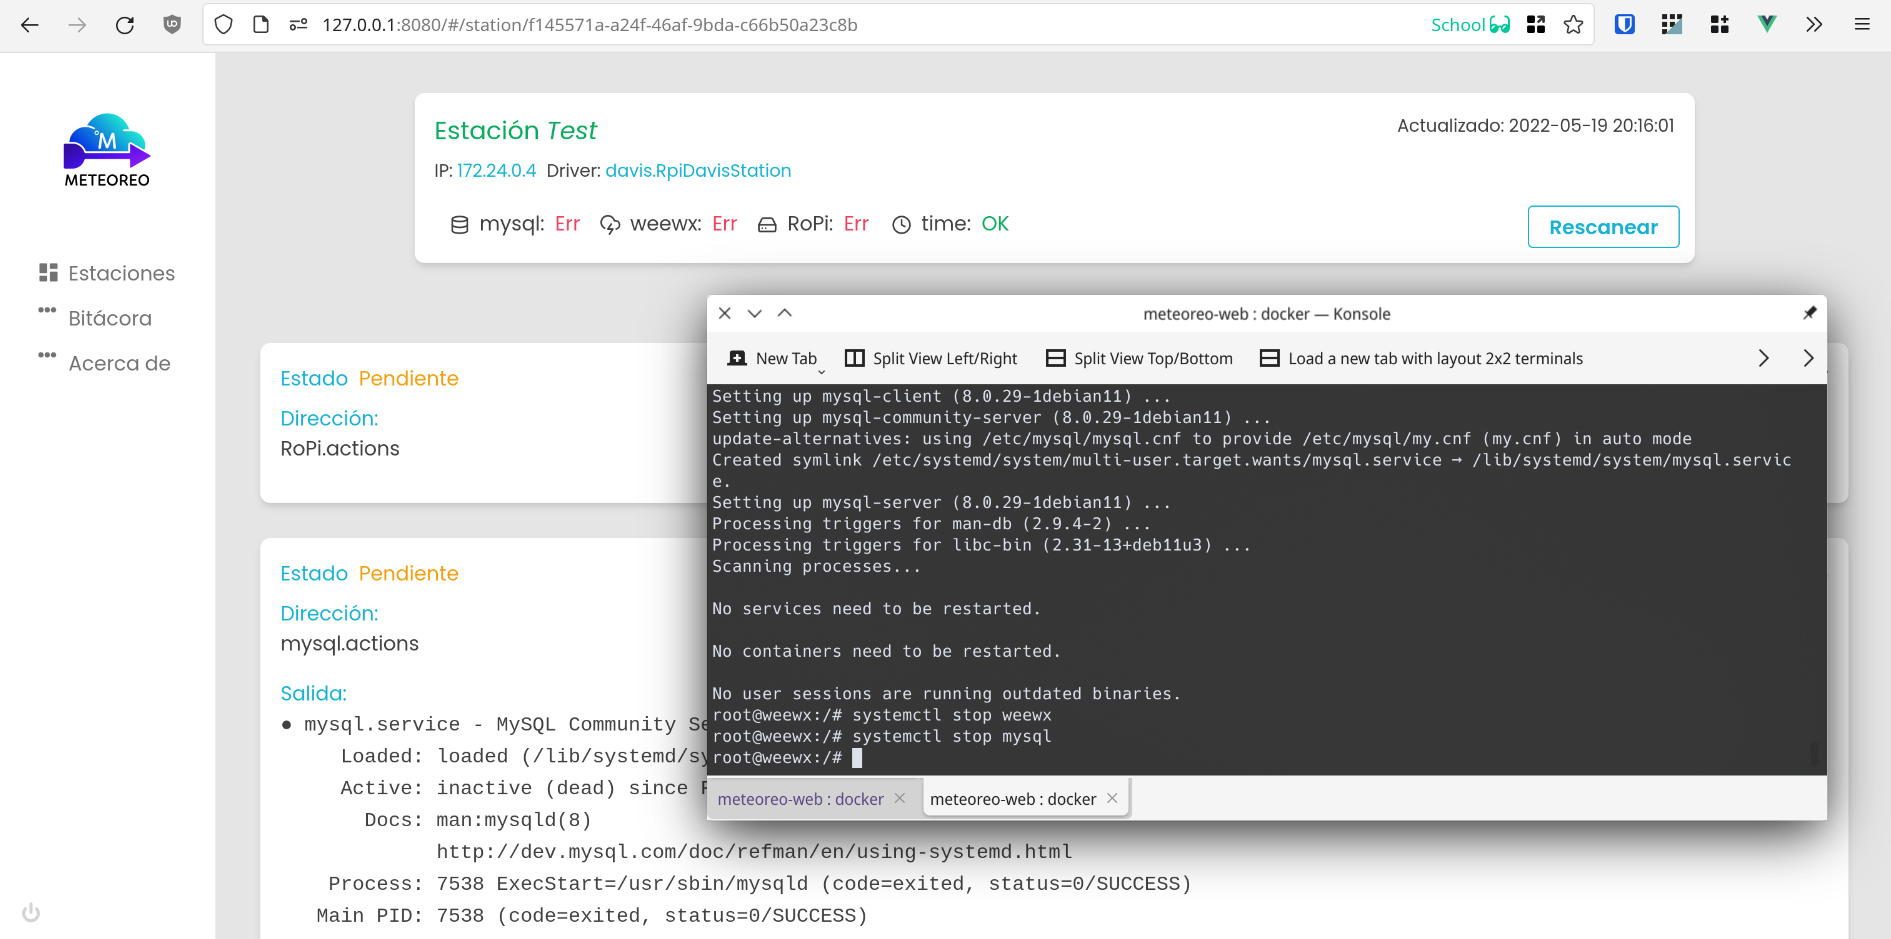
\includegraphics[width=1\linewidth]{images/screenshots/0.1.4-test_station_failed.png}
	\caption{Estado de en falla de la estación de prueba.}
	\label{fig:test-station-failed}
\end{figure}

Este resultado fué el esperado, ya que no existen configuraciones de fallas comunes para el estado detendo del servicio MySQL o WeeWX dado que estos pueden estar detenidos por una serie de razones impredecibles y no se ofrece el botón de acción de resolver estos errores, pero se da el detalle de este estado en la interfaz para facilitar el diagnóstico y retención de la información. Cuando los servicios en cuestión fueron vueltos a ejecutar, el sistema resolvió automáticamente los eventos y se mostró correctamente la información, con lo cual se dió por concluída la prueba, como puede observarse en la Figura \ref{fig:test-station-fixed}.

\begin{figure}[!ht]
	\centering
	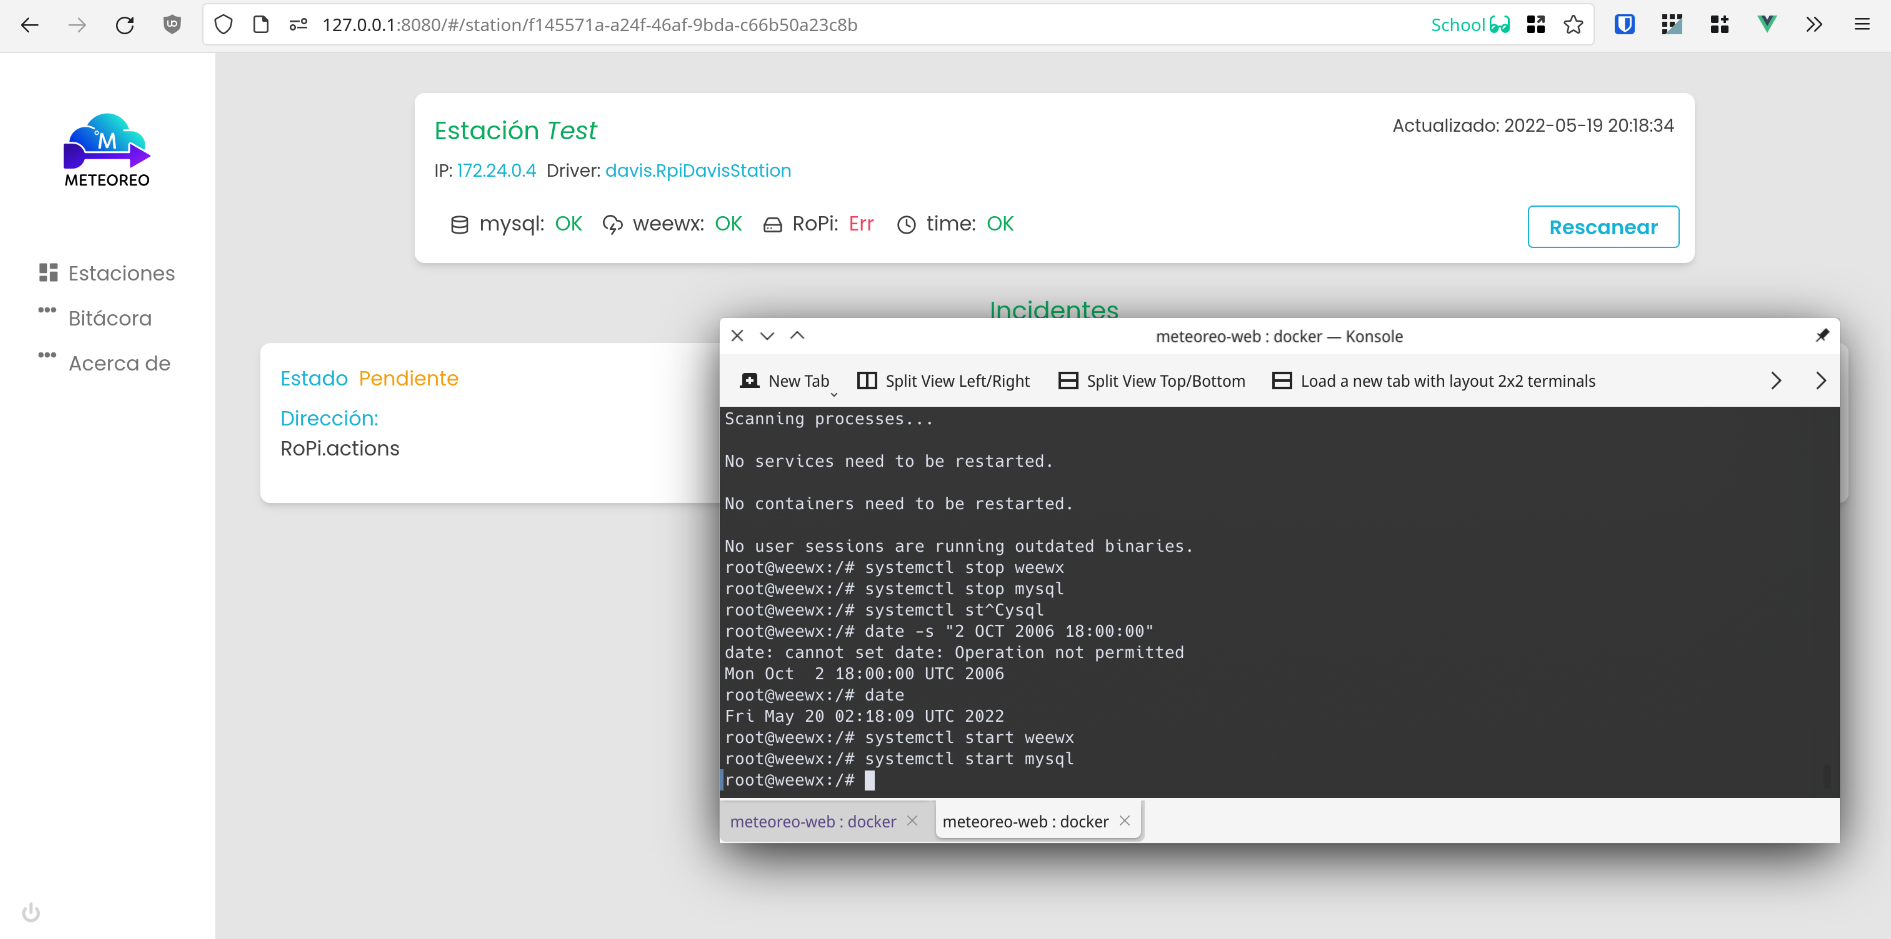
\includegraphics[width=1\linewidth]{images/screenshots/0.1.5-test_station_fixed.png}
	\caption{Estado final de la estación de prueba.}
	\label{fig:test-station-fixed}
\end{figure}

Además de esta prueba realizada se realizó un proceso similar, aunque menos invasivo, en la estación meteorológica ubicada en el Instituto de Ingeniería y Tecnología de la UACJ. Esta estación se eleigió debido a su alta disponibilidad y facilidad de diagnóstico ante un posible problema. En este caso, se hicieron pruebas con el servicio de RoPI, debido a que el impacto de su funcionamiento no ideal es negligible en un periodo corto de tiempo. Para esto, se realizó una conexión por SSH a la estación y se ejecutó el comando \texttt{sudo remountrw}, lo cual desactiva el modo sólo lectura. Después de ejecutarlo, se observó la interfaz gráfica para corroborar el correcto registro de este evento fué el previsto, como puede ser observado en la Figura \ref{fig:iit-ropi-disabled}.

\begin{figure}[!ht]
	\centering
	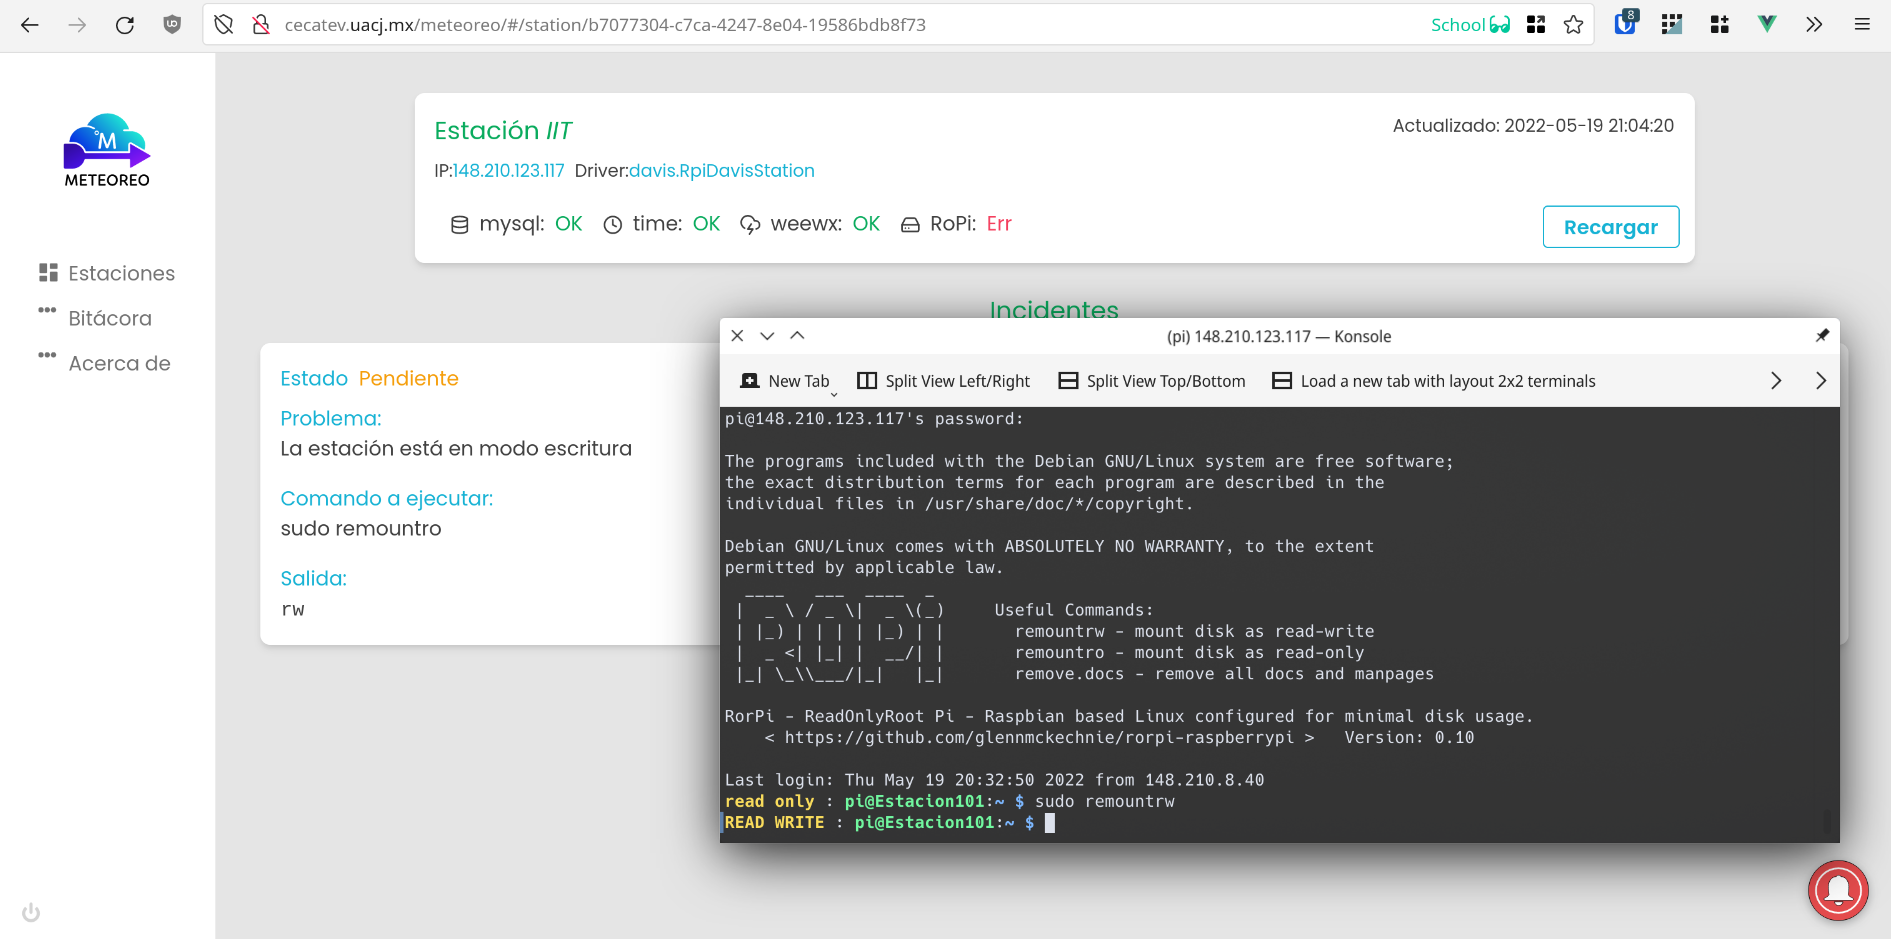
\includegraphics[width=1\linewidth]{images/screenshots/0.1.4-iit-ropi-disabled.png}
	\caption{Modo sólo lectura desactivado en la estación IIT.}
	\label{fig:iit-ropi-disabled}
\end{figure}

Al corroborarse que los resultados fueran los esperados, se presionó el botón de solución automática del error. Esto ejecutó el comando \texttt{sudo remountro}, como indica la tarjeta de error de servicio, en la estación meteorológica, y después de que el servicio de monitoreo detectara el cambio del estado, este fue reflejado correctamente en la interfaz, como se observa en la Figura \ref{fig:iit-ropi-fixed}. Con este resultado, y el resultado de la prueba anterior se determinó que el sistema era adecuado para su lanzamiento.

\begin{figure}[!ht]
	\centering
	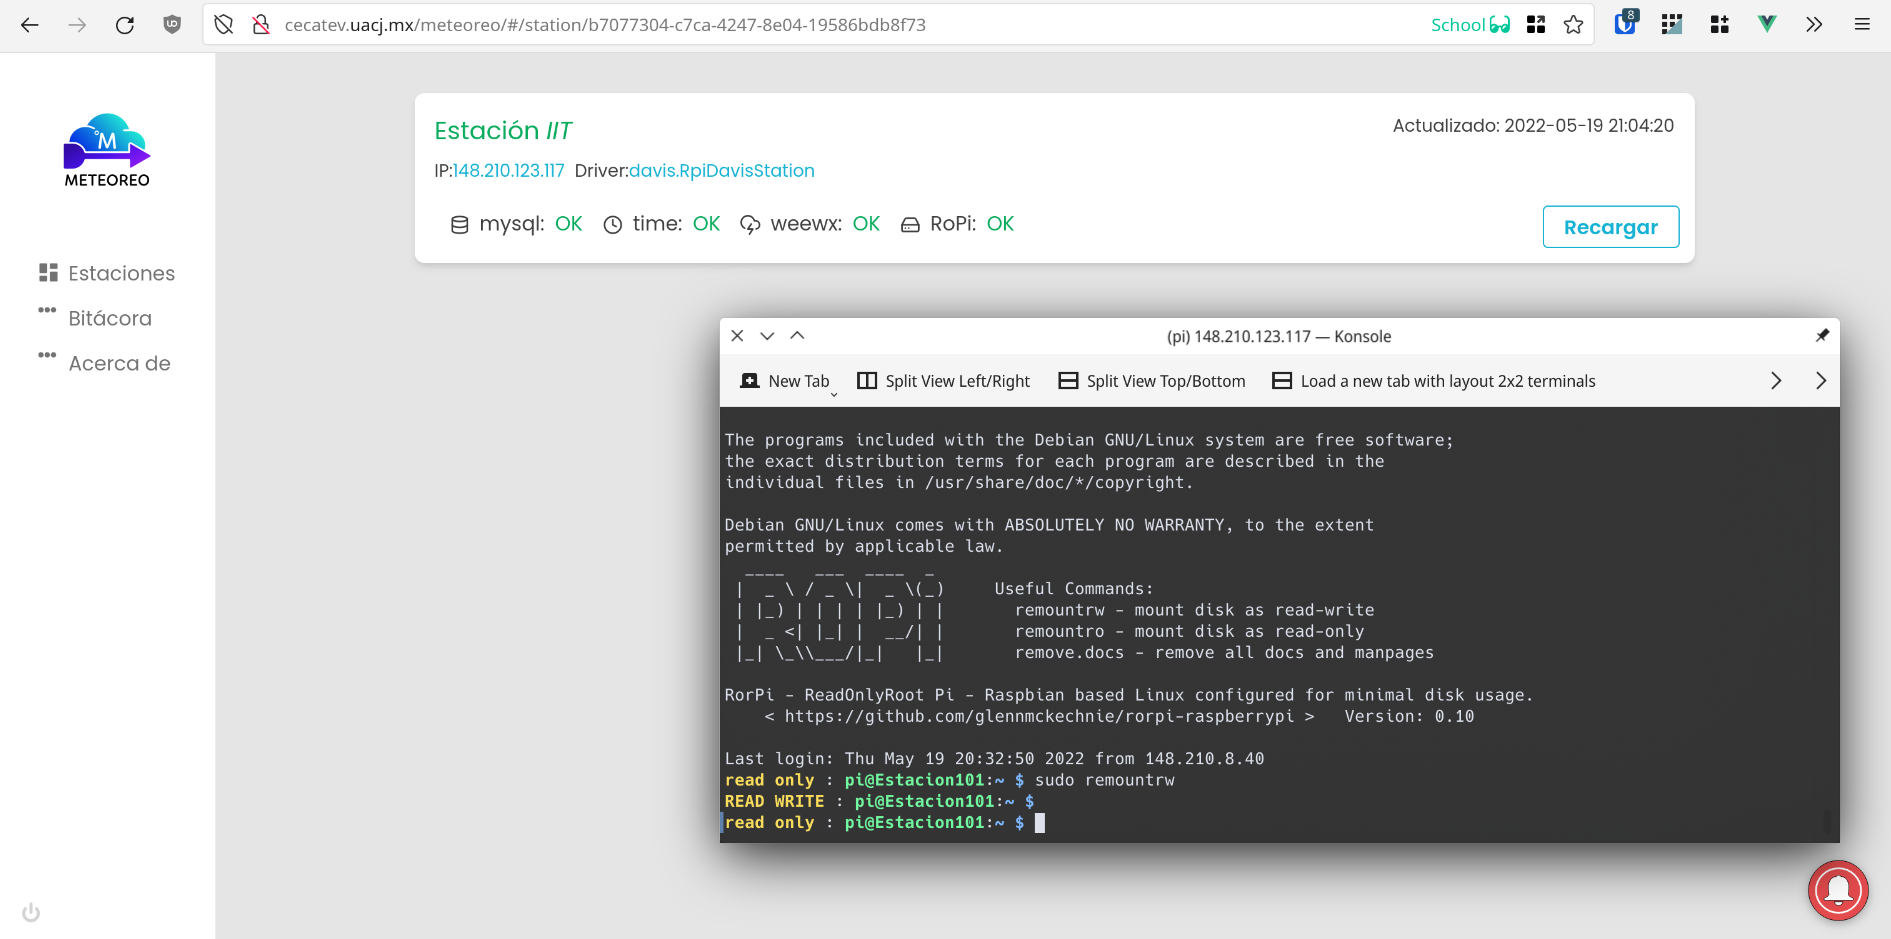
\includegraphics[width=1\linewidth]{images/screenshots/0.1.5-iit-ropi-fixed.png}
	\caption{Modo sólo lectura reactivado en la estación IIT.}
	\label{fig:iit-ropi-fixed}
\end{figure}

% https://github.com/instantlinux/docker-tools/blob/main/images/weewx/docker-compose.yml

% wget https://dev.mysql.com/get/mysql-apt-config_
% wget https://dev.mysql.com/get/mysql-apt-config_0.8.15-1_all.deb --no-check-certificate
% dpkg -i mysql-apt-config_0.8.15-1_all.deb

% wget https://dev.mysql.com/get/mysql-apt-config_0.8.22-1_all.deb --no-check-certificate
% apt-get install dialog apt-utils
% sudo dpkg -i mysql-apt-config_0.8.22-1_all.deb # Seleccionar mysql server
% apt-get update

% adduser pi;
% apt install sudo -y;
% visudo all users;
